\subsection{Clickable Plots}
\begin{pgfplotslibrary}{clickable}
	A library which generates small popups whenever one clicks into a plot. The popup displays the coordinate under the mouse pointer, supporting the optional snap--to--nearest |clickable coords| feature with customizable displayed information. Furthermore, the library allows to display slopes if one holds the mouse pressed and drags it to another point in the plot.

	The library has two purposes: to compute slopes in a simple way\footnote{The author is applied mathematician...} and to provide related, optional information to single data points which are not important enough to be listed in the main text (like prototype parameters or other technical things).
\end{pgfplotslibrary}


\subsubsection{Overview}
	It is completely sufficient to write 
\begin{codeexample}[code only]
\usepgfplotslibrary{clickable}
\end{codeexample}
	\noindent in the document preamble. This will automatically prepare every plot.

	The library works with Acrobat Javascript and \pdf\ forms: every plot becomes a push--button. 

	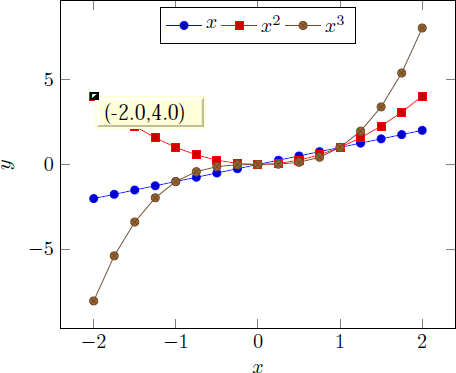
\includegraphics[height=6cm]{figures/pgfplotsclickable-fig1.png}
	\rlap{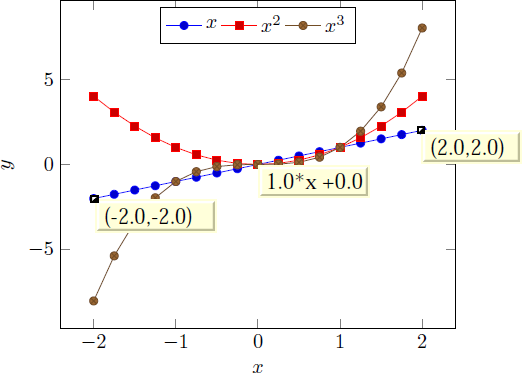
\includegraphics[height=6cm]{figures/pgfplotsclickable-fig2.png}}\hfill

	\nobreak
	These screenshots show the result of clicking into the axis range (left column) and of dragging from one point to another (right column). The second case shows the result of Drag-and-Drop: it displays start- and end points and the equation for the line segment between between the first point of the drag- and drop and the second point where the mouse has been released. The line segment is 
	\[ l(x; x_0,y_0,x_1,y_1) = m \cdot x + n \]
	where $m = (y_1-y_0) / (x_1-x_0)$ is the slope and $n$ the offset chosen such that $l(x_0;\dotsc) = y_0$. For logarithmic plots, logarithms will be applied before computing slopes. 

	\noindent
	\hbox to \linewidth{%
	\hspace{-0.5cm}%
	\begin{tikzpicture}
		\node at (8cm,0cm)	{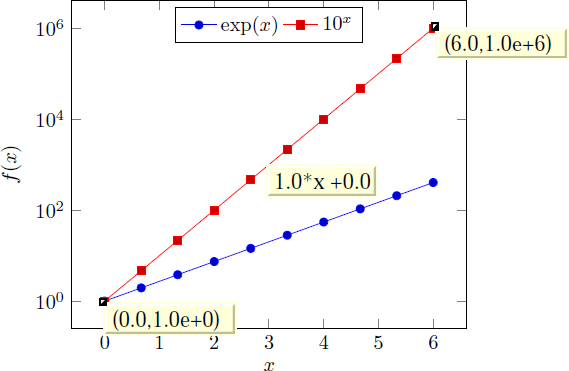
\includegraphics[height=6cm]{figures/pgfplotsclickable-fig4.png}};
		\node at (0cm,0cm)	{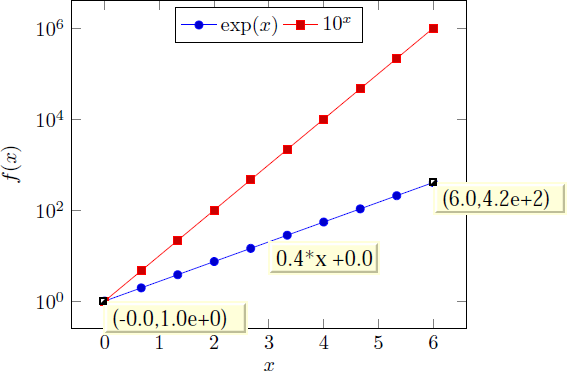
\includegraphics[height=6cm]{figures/pgfplotsclickable-fig3.png}};
	\end{tikzpicture}\hss}%

	\nobreak
	These screen shots show the result of drag- and drop for \emph{logarithmic} axes: the end points show, again, the coordinates (without logs) and the form field in the middle shows the slope and offset of the linear equation in log coordinates.

	The log basis for any logarithmic axes is usually~$10$, but it respects the current setting of |log basis x| and |log basis y|. The applied log will always use the same logarithm which is also used for the axis descriptions (this is not necessarily the same as used by \PGFPlotstable!).

	This document has been produced with the |clickable| library, so it is possible to load it into Acrobat Reader and simply click into a plot.
	
	\expandafter\ifx\csname pgfplotsclickabledisabled\endcsname\relax
	\else
	\paragraph{Attention:} For this document, the |clickable| library has been deactivated. You may find a different version on \url{http://sourceforge.net/projects/pgfplots}.
	\fi

\begin{pgfplotskey}{clickable coords=\marg{displayed text}}
	Activates a snap--to--nearest feature when clicking onto plot coordinates. The \meta{displayed text} is the coordinate's $x$ and $y$ value by default (i.e.\ you write just |clickable coords| without an equal sign).
\begin{codeexample}[]
\begin{tikzpicture}
	\begin{loglogaxis}[clickable coords=
		{Level \thisrow{level} (q=\thisrow{q})}]
	\addplot table[x=dof,y=error] {
level  dof     error           q      
1      4       2.50000000e-01  48        
2      16      6.25000000e-02  25        
3      64      1.56250000e-02  41        
4      256     3.90625000e-03  8         
5      1024    9.76562500e-04  22        
6      4096    2.44140625e-04  46        
7      16384   6.10351562e-05  40        
8      65536   1.52587891e-05  3
9      262144  3.81469727e-06  1
10     1048576 9.53674316e-07  9
	};
		
	\end{loglogaxis}
\end{tikzpicture}
\end{codeexample}
	\noindent Now, clicking onto a data point yields `Level 7 (q=40)' 
	whereas clicking besides a data point results in the click coordinates as before,
	
	\noindent\hbox to \linewidth{\hfill
	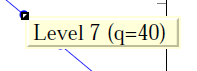
\includegraphics[scale=0.4]{figures/pgfplotsclickable-log-snap0}\hfill
	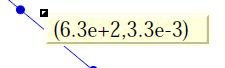
\includegraphics[scale=0.4]{figures/pgfplotsclickable-log-snap2}\hfill
	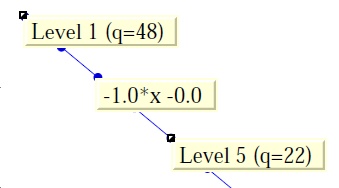
\includegraphics[scale=0.4]{figures/pgfplotsclickable-log-snap1}.\hfill
	}%

	Note that logarithmic slopes work as before.
	
	If you want the $(x,y)$ values to be displayed, use the special placeholder string `|(xy)|' inside of \meta{displayed text}. As an example, we consider again the |scatter/classes| example of page~\pageref{pgfplots:scatterclasses}:

\begin{codeexample}[]
\begin{tikzpicture}
	\begin{axis}[%
	clickable coords={(xy): \thisrow{label}},%
	scatter/classes={%
		a={mark=square*,blue},%
		b={mark=triangle*,red},%
		c={mark=o,draw=black}}]
	\addplot[scatter,only marks,%
		scatter src=explicit symbolic]%
	table[meta=label] {
x     y      label
0.1   0.15   a 
0.45  0.27   c 
0.02  0.17   a 
0.06  0.1    a 
0.9   0.5    b 
0.5   0.3    c 
0.85  0.52   b 
0.12  0.05   a 
0.73  0.45   b 
0.53  0.25   c 
0.76  0.5    b 
0.55  0.32   c
	};
	\end{axis}
\end{tikzpicture}
\end{codeexample}
	\noindent Here, we find popups like

	\noindent\hbox to \linewidth{\hfill
	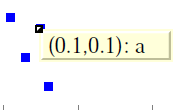
\includegraphics[scale=0.4]{figures/pgfplotsclickable-scatter1.png}\hfill
	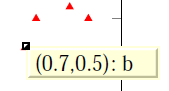
\includegraphics[scale=0.4]{figures/pgfplotsclickable-scatter2.png}\hfill
	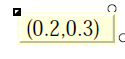
\includegraphics[scale=0.4]{figures/pgfplotsclickable-scatter0.png}.\hfill
	}%

	The \meta{displayed text} is a richtext string displayed with \emph{Javascript}. For most purposes, it is used like an unformatted C string: it contains characters, perhaps line breaks with `|\n|' or tabulators with `|\t|', but it should not contain \TeX\ formatting instructions, especially no math mode (the `|(xy)|' replacement text is formatted with |sprintf|, see below). Consider |clickable coords code| in case you'd like to preprocess data before displaying it. If you experience problems with special characters, try prepending a backslash to them. If that doesn't work either, try to prefix the word with `|\\|' and/or with `|\string|'. Consider using |clickable coords size| if you intend to work with multiline fields and the size allocation needs improvements.

	In fact, \meta{displayed text} can even contain richtext (=XHTML) formatting instructions like `|<br/>|' (note the final slash) or `|<span style="color:\#7E0000;">text</span>|' (note the backslash before `|#|') which changes the color for |text|. The |<span style="">| arguments are CSS fields, consider an HTML reference for a list of CSS attributes.

	It is possible to use |clickable coords| together with three dimensional axes. Note that dynamic (clickable) features of a three dimensional axis without |clickable coords| will be disabled (they appear to be useless). Furthermore, three dimensional axes do not support slope calculations; only the snap--to--nearest feature is available.

	Consider using |annot/snap dist=6| to increase the snap--to--nearest distance.

	The |clickable coords| can be specified for all plots in an axis (as in the examples above), but also once for every single |\addplot| commands for which the snap--to--nearest feature is desired (with different \meta{displayed text}). 

	If multiple |clickable coords| are on the same position, each click chooses the next one (in the order of appearance).
\end{pgfplotskey}

\begin{pgfplotskey}{clickable coords code=\marg{\TeX\ code which defines {\normalfont\ttfamily\textbackslash pgfplotsretval}}}
	A variant of |clickable coords| which allows to prepare the displayed information before it is handed over to Javascript.

	The value should be \TeX\ code which defines |\pgfplotsretval| somehow. The result is used as simple, unformatted string which is associated to coordinates.

	Consider using 
	
	\hspace{2em}|\pgfmathprintnumberto[verbatim]|\marg{number}|\macroname|
	
	\hspace{2em}|\edef\pgfplotsretval{Number=\macroname}|
	
	to provide number printing. The |\pgfmathprintnumberto[verbatim]| doesn't use math mode to format a number\footnote{See the \PGFPlotstable\ manual for details about number printing.}, and it writes its result into |\macroname|. The name `|\macroname|' is arbitrary, use anything like `|\eps|' or `|\info|'. The |\edef| means ``expanded definition'' and has the effect of expanding all macros to determine the value, in our case ``Number= \meta{the value}''. The following example uses it twice to pretty--print the data:
\begin{codeexample}[]
\begin{tikzpicture}
\begin{loglogaxis}[clickable coords code={%
	\pgfmathprintnumberto[verbatim,precision=1]%
		{\thisrow{error}}%
		\error%
	\pgfmathprintnumberto[verbatim,frac]%
		{\thisrow{frac}}%
		\fraccomp%
	\edef\pgfplotsretval{error \error, R=\fraccomp}%
}]%
\addplot table[x=dof,y=error] {
level  dof     error           frac      
1      4       2.50000000e-01  0.5        
2      16      6.25000000e-02  0.75      
3      64      1.56250000e-02  0.1        
4      256     3.90625000e-03  0.2         
5      1024    9.76562500e-04  0.5        
6      4096    2.44140625e-04  0.8        
7      16384   6.10351562e-05  0.125        
8      65536   1.52587891e-05  0.725
9      262144  3.81469727e-06  0.625
10     1048576 9.53674316e-07  1
};
	
\end{loglogaxis}
\end{tikzpicture}
\end{codeexample}
	\noindent resulting in

	\noindent\hbox to \linewidth{\hfill
	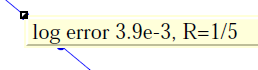
\includegraphics[scale=0.4]{figures/pgfplotsclickable-logcode-snap0.png}\hfill
	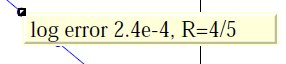
\includegraphics[scale=0.4]{figures/pgfplotsclickable-logcode-snap1.png}.\hfill
	}%

	The \meta{\TeX\ code} is evaluated inside of a local scope, all locally declared variables are freed afterwards (that's why you can use any names you want).
\end{pgfplotskey}

\begin{pgfplotskey}{clickable coords size=\texttt{auto} or \marg{max chars} or \marg{max chars x,max chars y} (initially auto)}
	This is actually just another name for |annot/popup size snap|, see its documentation below.
\end{pgfplotskey}

\subsubsection{Requirements for the Library}
	\begin{itemize}
		\item The library relies on the \LaTeX\ packages |insdljs| (``Insert document level Javascript'') and |eforms| which are both part of the freely available |AcroTeX| education bundle~\cite{acrotex}\footnote{These packages rely on \LaTeX, so the library is only available for \LaTeX, not for plain \TeX\ or Con\TeX t.}. The |insdljs| package creates a temporary file with extension |.djs|.
		
		\item At the time of this writing, only Adobe Acrobat Reader interpretes Javascript and Forms properly. The library doesn't have any effect if the resulting document is used in other viewers (as far as I know).

	\end{itemize}
	Note that although this library has been written for \PGFPlots, it can be used independently of a \PGFPlots\ environment.

	\paragraph{Compatibility issues:}
	There a several restrictions when using this library. Most of them will vanish in future versions -- but up to now, I can't do magic.
	\begin{itemize}
		\item The library does not yet support rotated axes. Use |clickable=false| for those axes.
		\item The library works only with |pdflatex|; |dvips| or |dvipdfm| are not supported\footnote{In fact, they should be. I don't really know why they don't $\hdots$ any hint is welcome.}.

		\item Up to now, it is \emph{not} possible to use this library together with the |external| library and other image externalization methods of Section~\ref{sec:pgfplots:importexport}.
		
		To be more precise, you can (with two extra preamble lines, see below) get correctly annotated, exported \pdf\ documents, but the |\includegraphics| command does not import the dynamic features.

		In case you decide to use this work--around, you need to insert
\begin{codeexample}[code only]
% \maxdeadcycles=10000 % in case you get the error `Output loop---<N> consecutive dead cycles.'
\usepackage[pdftex]{eforms}	
\end{codeexample}
		\noindent \emph{before} loading \pgfname, \Tikz\ or \PGFPlots. The |\maxdeadcycles| appears to be necessary for large documents, try it out.

		As long as you are working on a draft version of your document, you might want to use
\begin{codeexample}[code only]
\pgfkeys{/pgf/images/include external/.code={\href{file:#1}{\pgfimage{#1}}}}
\end{codeexample}
		in your preamble. This will generate hyperlinks around the graphics files which link to the exported figures. Clicking on the hyperlinks opens the exported figure which, in turn, has been generated with the |clickable| library and allows dynamic features\footnote{This special treatment needs the external files in the same base directory as the main document, so this approach is most certainly \emph{not} suitable for a final document.}.


		\item The library automatically calls |\begin{Form}| at |\begin{document}| and |\end{Form}| at the end of the document. This environment of |hyperref| is necessary for dynamic user interaction and should be kept in mind if the document contains other form elements.
	\end{itemize}

	\paragraph{Acknowledgements:}
	\begin{itemize}
		\item I have used a Javascript |sprintf| implementation of Kevin van Zonneveld~\cite{phptojs} (the Javascript API has only a limited set of conversions).
	\end{itemize}


\subsubsection{Customization}
It is possible to customize the library with several options.

\begin{pgfplotskey}{clickable=\mchoice{true,false} (initially true)}
	Allows to disable the library for single plots.
\end{pgfplotskey}

\begin{pgfplotskey}{annot/js fillColor=\marg{Javascript color} (initially ["RGB",1,1,.855])}
	Sets the background (fill) color of the short popup annotations. 
	
	Possible choices are |transparent|, gray, RGB or CMYK color specified as four--element--arrays of the form
	|["RGB", |\meta{red}|,|\meta{green}|,|\meta{blue}|]|. Each color component is between $0$ and $1$.

	Again: this option is for Javascript. It is \emph{not} possible to use colors as in \pgfname.
\end{pgfplotskey}

\begin{pgfplotskeylist}{%
	annot/point format=\marg{sprintf-format} (initially {(\%.1f,\%.1f)}),
	annot/point format 3d=\marg{sprintf-format} (initially {(\%.1f,\%.1f,\%.1f)})}
	Allows to provide an |sprintf| format string which is used to fill the annotations with text. 
	The first argument to |sprintf| is the $x$-coordinate and the second argument is the $y$-coordinate.

	The |point format 3d| variant is used for any three--dimensional axis whereas the |point format| is used (only) for two--dimensional ones.

	The |every semilogx axis|, |every semilogy axis| and |every loglog axis| styles have been updated to
\begin{codeexample}[code only]
\pgfplotsset{
	every semilogy axis/.append style={/pgfplots/annot/point format={(\%.1f,\%.1e)}},
	every semilogx axis/.append style={/pgfplots/annot/point format={(\%.1e,\%.1f)}},
	every loglog axis/.append style={/pgfplots/annot/point format={(\%.1e,\%.1e)}}
}
\end{codeexample}
	\noindent such that every logarithmic coordinate is displayed in scientific format.
\end{pgfplotskeylist}

\begin{pgfplotskey}{annot/slope format=\marg{sprintf-format} (initially \%.1f*x \%+.1f)}
	Allows to provide an |sprintf| format string which is used to fill the slope--annotation with text.
	The first argument is the slope and the second the line offset.
\end{pgfplotskey}

\begin{pgfplotskey}{annot/printable=\mchoice{true,false} (initially false)}
	Allows to configure whether the small annotations will be printed. Otherwise, they are only available on screen.
\end{pgfplotskey}

\begin{pgfplotskey}{annot/font=\marg{Javascript font name} (initially font.Times)}
	Allows to choose a Javascript font for the annotations. Possible choices are limited to what Javascript accepts (which is \emph{not} the same as \LaTeX). The default fonts and its names are shown below.

	\begin{center}
	\begin{tabular}{ll}
		\toprule
		Font Name	& Name in Javascript\\
		\midrule
		Times-Roman           & font.Times\\
        Times-Bold            & font.TimesB\\
        Times-Italic          & font.TimesI\\
        Times-BoldItalic      & font.TimesBI\\
        Helvetica             & font.Helv\\
        Helvetica-Bold        & font.HelvB\\
        Helvetica-Oblique     & font.HelvI\\
        Helvetica-BoldOblique & font.HelvBI\\
        Courier               & font.Cour\\
        Courier-Bold          & font.CourB\\
        Courier-Oblique       & font.CourI\\
        Courier-BoldOblique   & font.CourBI\\
        Symbol                & font.Symbol\\
        ZapfDingbats          & font.ZapfD\\
		\bottomrule
	\end{tabular}
	\end{center}
\end{pgfplotskey}

\begin{pgfplotskey}{annot/textSize=\marg{Size in Point} (initially 11)}
	Sets the text size of annotations in points.
\end{pgfplotskey}

\begin{pgfplotskeylist}{%
	annot/popup size generic=\texttt{auto} or \marg{x} or \marg{x,y} (initially auto),%
	annot/popup size snap=\texttt{auto} or \marg{x} or \marg{x,y} (initially auto),%
	annot/popup size=\marg{value}}%
	The first key defines the size of popups if you just click into an axis. The second key defines the size of popups for the snap--to--nearest feature (i.e.\ those prepared by |clickable coords|). The third key sets both to the same \meta{value}.

	The argument can be |auto| in which case \PGFPlots\ tries to be smart and counts characters. This may fail for multiline texts. The choice \meta{x} provides the \emph{horizontal} size only, in units of |annot/textSize|. Thus, |annot/popup size generic=6| makes the popup $6\cdot 11$ points wide. In this case, only one line will be allocated. Finally, \meta{x,y} allows to provide horizontal and vertical size, both in units of |annot/textSize|.

	See also |clickable coords size| which is an alias for |annot/popup size snap|.
\end{pgfplotskeylist}


\begin{pgfplotskey}{annot/snap dist=\marg{Size in Point} (initially 4)}
	Defines the size within two mouse clicks are considered to be equivalent, meased in points (Euclidean distance).
\end{pgfplotskey}

\begin{pgfplotskey}{annot/richtext=\mchoice{true,false} (initially true)}
	Enables or disables richtext formatting in |clickable coords| arguments. Richtext is kind of XHTML and allows CSS styles like colors, font changes and other CSS attributes, see the documentation for |clickable coords| for details.

	The case |annot/richtext=false| is probably more robust.
\end{pgfplotskey}

\subsubsection{Using the Clickable Library in Other Contexts}
This library provides essentially one command, |\pgfplotsclickablecreate| which creates a clickable area of predefined size, combined with Javascript interaction code. It can be used independently of \PGFPlots.

\begin{command}{\pgfplotsclickablecreate\oarg{required key-value-options}}
	Creates an area which is clickable. A click produces a popup which
	contains information about the point under the cursor.
	
	The complete (!) context needs to be provided using key-value-pairs, either set before
	calling this method of inside of \oarg{required key-value-options}.
	
	This command actually creates an AcroForm which invokes Javascript
	whenever it is clicked. A Javascript Object is created which
	represents the context (axis limits and options). This Javascript
	object is available at runtime.
	
	This method is public and it is \emph{not} restricted to \PGFPlots.
	The \PGFPlots\ hook simply initializes the required key-value-pairs.

	This method does not draw anything. It initializes only a
	clickable area and Javascript code.
	
	The required key-value-pairs are documented below.
	
	\paragraph{Attention:} Complete key-value validation is \emph{not} performed here. It
	can happen that invalid options will produce Javascript bugs when
	opened with Acrobat Reader. Use the Javascript console to find them.
\end{command}

\noindent All options described in the following are only interesting for users who intend to use this library without \PGFPlots.

\begin{pgfplotskey}{annot/width=\marg{dimension} (initially -)}
	This required key communicates the area's width to |\pgfplotsclickablecreate|. It must be a \TeX\ dimension like |5cm|.
\end{pgfplotskey}
\begin{pgfplotskey}{annot/height=\marg{dimension} (initially -)}
	This required key communicates the area's height to |\pgfplotsclickablecreate|. It must be a \TeX\ dimension like |5cm|.
\end{pgfplotskey}
\begin{pgfplotskey}{annot/jsname=\marg{string} (initially -)}
	This required key communicates a unique identifier to |\pgfplotsclickablecreate|. This identifier is used to identify the object in Javascript, so there can't be more than one of them. If it is empty, a default identifier will be generated.
\end{pgfplotskey}

\begin{pgfplotskeylist}{annot/xmin=\marg{number},annot/xmax=\marg{number},annot/ymin=\marg{number},annot/ymax=\marg{number} (initially empty)}
	These required keys communicate the axis limits to |\pgfplotsclickablecreate|. They should be set to numbers which can be assigned to a Javascript floating point number (standard IEEE double precision).
\end{pgfplotskeylist}

\begin{pgfplotskey}{annot/collected plots=\marg{nested arrays} (initially empty)}
	The low level interface to implement a snap--to--nearest feature. The value is an array of plots, where each plot is again an array of coordinates and each coordinate is an array of three elements, $x$, $y$ and text. Please consult the code comments for details and examples.
\end{pgfplotskey}
